\chapter{Travail réalisé}
    \section{Mon travail}
    % Présentation du travail a effectuer sur le projet.
    \begin{flushleft}
        Avant de commencer, je vous présente mon travail sur le sujet du stage.

        \vspace{0.2cm}
    
        Dans un premier temps, il faudra installer le système Raspbian.
        Une fois l'installation faire, il faudra configurer le système.
        Avant de commencer l'application, il me faudra faire quelques tests afin de vérifier le bon fonctionnement.
        Une fois cela terminé, il me faut vérifier que la caméra fonctionne correctement.    
    \end{flushleft}

    \section{Présentation du Matérriel}
        \subsection{Raspberry Pi}
        Le \textit{Raspberry Pi} est un ordinateur portable de petite taille, doté d'un processeur ARM et d'un système d'exploitation Linux.
        \begin{figure}[h]
            \centering
            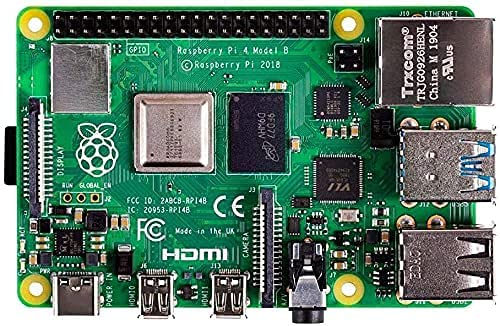
\includegraphics[scale=0.2]{rasp.jpg}
            \caption{Raspberry Pi 4}
        \end{figure}

        \subsection{Ecran LCD (Raspberry Pi) tailles}
        Avec le \textit{Raspberry Pi} un écran LCD de 7 pouces permettant d'interagir avec l'ordinateur grâce à son écran tactile. 
        \begin{figure}[h]
            \centering
            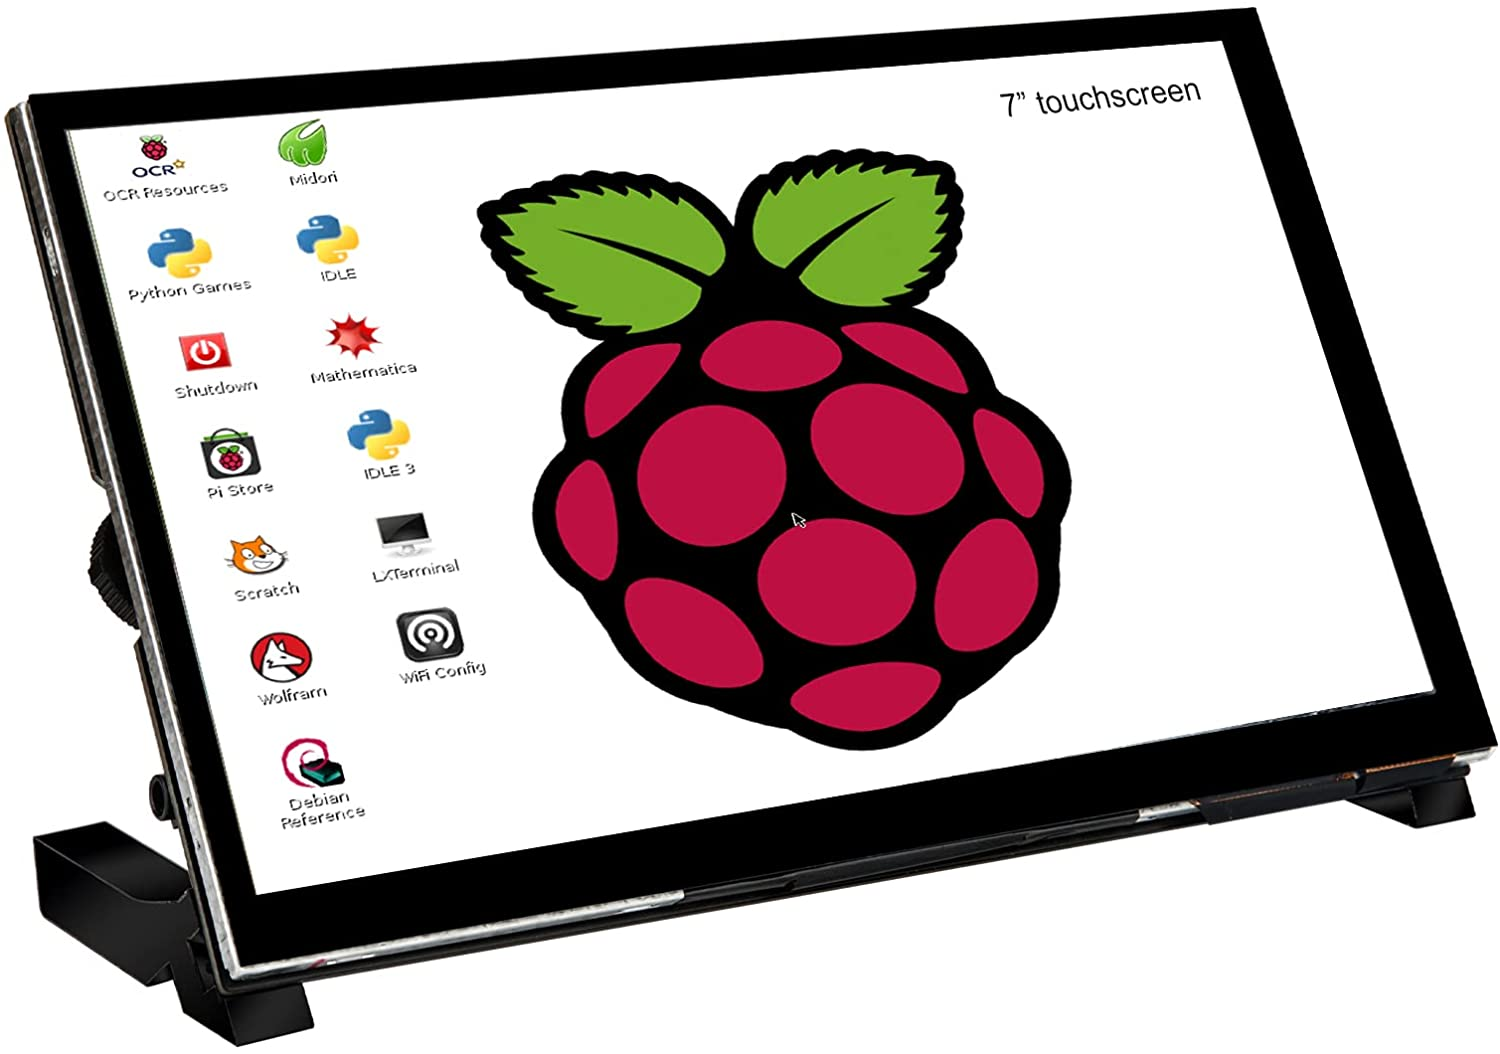
\includegraphics[scale=0.05]{ecran7p.jpg} 
            \caption{Ecran LCD de 7 pouces}
        \end{figure}

        \vspace{1cm}

        \subsection{Module de capture vidéo (Raspberry Pi) V2}
        Le module de capture vidéo (Raspberry Pi) V2 est un module de captation vidéo qui permet de capturer des images et des vidéos.
        \begin{figure}[h]
            \centering        
            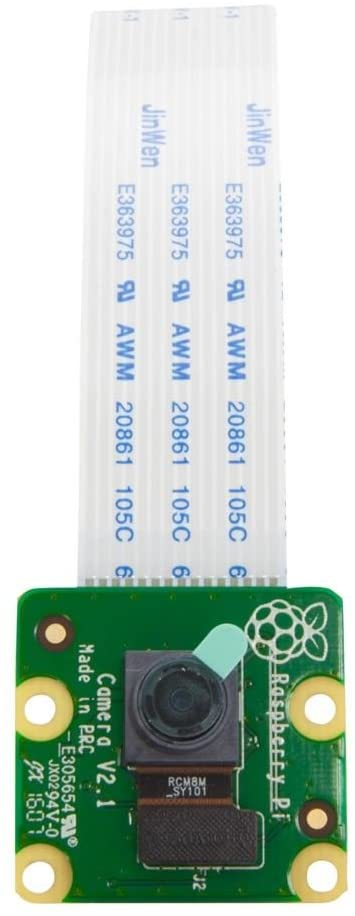
\includegraphics[scale=0.1]{module_cam.jpg}
            \caption{Module de capture vidéo (Raspberry Pi) V2}
        \end{figure}
        
    \section{Montage, Installation et Configuration}
        \subsection{Installation du matériel}  
        \subsection{Configuration du matériel}
    \section{Choix des technologies}
    Pour le choix du langage de programmation, je me suis basé sur les langages de programmation les plus classés pour le (Raspberry Pi) système d'exploitation Raspbian.
    Lors de ma recherche 5 langages de programmation en sont sortis : 

    \vspace{0.2cm}

    \begin{itemize}
        \item Python
        \item C
        \item Java/BlueJ
        \item Perl
        \item Scratch
    \end{itemize}

    \vspace{0.2cm}

    \begin{flushleft}
        Ainsi que la disponibilité d'une API afin de pouvoir utiliser la caméra.
        J'ai donc fait le choix de l'API PiCamera car c'est celle qui est par défaut installée sur le Raspberry Pi donc nativement compatible avec la caméra.\\[0.2cm]
    
        Même si le langage de programmation JavaScript ne figure pas dans cette liste, il est très utilisé, il est donc très intéressant de le choisir.
        Avec electron et nodejs, nous pouvons très bien créer une application multiplatforme.\\[0.2cm]
        De plus, l'API PiCamera est disponible pour le langage JavaScript.
    
        Mais par manque de temps, nodejs et electron ne sont pas installés par défaut sur le Raspberry Pi.\\[0.2cm]
    
        De ce fait nous allons utiliser le langage Python pour la programmation du logiciel.
        Le Pi dans "Raspberry Pi" signifie "Python". Il a le mérite d'être le choix par défaut, il est installé par défaut sur le Raspberry Pi et le module PiCamera est disponible.\\[0.2cm]
    
        Donc je vais utiliser le langage Python pour la programmation du logiciel et l'API PiCamera pour la capture vidéo.
    \end{flushleft}

    % Qu'est ce que le langage Python ?
    
    \section{Réalisation de l'application}
        
        